\chapter{Introducción}
  Se le llama reloj de agua o clepsidra \textemdash del griego \foreignlanguage{greek}{κλέπτειν} \textit{kleptein}
  ``robar'', \foreignlanguage{greek}{ὕδωρ} \textit{hydor}, ``agua''\textemdash a cualquier reloj que
  mida el tiempo mediante un flujo regulado de líquido hacia o
  desde un recipiente. Se considera como el instrumento de medición de tiempo
  más antiguo de la historia, y aunque no se sabe dónde ni cuando se
  inventaron, se han encontrado indicios de estos instrumentos en la antigua
  Babilonia y Egipto \textemdash Siglo XVI a.C. \textemdash, India y China \textemdash
  incluso algunos autores afirman que apareció en china en el año 4.000 a.C.\textemdash.
  Más adelante los griegos y los romanos mejorarían los relojes de agua introduciendo
  un ingenioso sistema que aumentaría la precisión de estos instrumentos considerablemente.\cite{clepsidra_wiki}

\section{Contexto de la empresa}
\label{context:company}

GuGo Creative S.L. es una empresa emergente localizada en Donostia, la
cual centra su actividad en el diseño y desarrollo tanto de soluciones web
como de aplicaciones móviles.

\section{Motivación del proyecto propuesto y objetivos}
La empresa utilizaba una aplicación de seguimiento y control de tiempos,
que permitía dar de alta clientes, proyectos y tareas, y que recogía
las imputaciones de tiempo que los trabajadores dedicaban a cada
proyecto. El objetivo era generar un informe para después exportarlo,
y mediante un programa externo obtener las rentabilidades de los
proyectos y los clientes.

Según se me informó, dicha aplicación la escogieron después de hacer un
estudio de las diferentes alternativas existentes, pero aún y todo, no
suplía todas las necesidades específicas de la empresa y además, tenía
funcionalidades que no se utilizaban en absoluto.

Por todo ello, se propuso realizar un desarrollo propio, el cual
supliera las necesidades que tenía la empresa, y fuera suficientemente
extensible o modificable para poder comercializar el producto para otras
empresas. También se pretendía que las diferentes capas \textemdash capa
de presentación, lógica de negocio y acceso a datos \textemdash fueran
independientes para facilitar el desarrollo de diferentes capas de 
presentación que pudieran hacer uso de la aplicación: una capa
web, móvil o de aplicación de escritorio.



\chapter{Gestión del proyecto}

\section{Gestión del alcance del proyecto}
La propuesta del proyecto incluye unas indicaciones generales de cómo quiere
la empresa que sea la aplicación, pero son insuficientes para poder realizar
un análisis realista del alcance que va a tener el proyecto.

Además, hay que tener en cuenta que el objetivo de este proyecto es realizar
una aplicación que funcione de forma cohesionada entre los diferentes
departamentos de la empresa, por lo que es muy probable que las
requerimientos cambien a lo largo del desarrollo del proyecto, o se tengan
que modificar.

\subsection{Planificación de la gestión del alcance}
El alcance del proyecto se generará una vez se conozcan, validen y contrasten
todos los requerimientos recogidos. Después, se generará la \gls{edt} una vez
se disponga de la primera versión del alcance, e incluirá todos los aspectos
del \gls{pfm}: planificación, gestión, desarrollo, seguimiento y control y
cierre.

El seguimiento y control del alcance se realizará a lo largo del desarrollo
del proyecto, revisando también los requerimientos, para evaluar si será
necesaria la aplicación de una modificación al alcance y al \gls{edt}. Antes de
hacer efectiva una modificación se tendrá que evaluar y comprobar que la
aplicación de dicha modificación no afecte a la viabilidad del proyecto.
Seguidamente se comprobará el \gls{edt} y se verificará si es necesario también
un cambio en dicha estructura.

\subsection{Planificación de la gestión de requerimientos}
\label{subsec:pgr}
Los trabajadores usan actualmente una aplicación determinada de seguimiento y
control de tiempos, clientes y proyectos. Es por ello que es crucial realizar
entrevistas con los trabajadores de los diferentes departamentos para extraer
de sus respuestas aquellas cosas que les gustan, las que no, y las que
mejorarían, además de su experiencia en general usando dicha aplicación. Al
procesar estas respuestas se podrán obtener los requerimientos del producto
a desarrollar y, finalmente, su validación consistirá en exponer dichos
requerimientos ante los interesados del proyecto, dando su visto bueno o no
a aquellos puntos con los que estén de acuerdo.

El seguimiento y control de los requerimientos se realizará a lo largo del
desarrollo del proyecto, cuando los diferentes interesados de la aplicación
contrasten que los requerimientos indicados y las que finalmente han sido
implementadas coinciden.

En caso de que los requerimientos tengan que sufrir algún cambio, se
evaluará si el nuevo requerimiento, o la modificación de uno ya existente,
es viable y se puede llevar a cabo. Se podrá modificar la prioridad e
importancia de los diferentes requerimientos, e incluso descartar unos
requerimientos por otros. En caso de que los cambios en los requerimientos
supongan un cambio drástico en el proyecto, se realizará una reunión con
los interesados del proyecto para ratificar dicho cambio.

\subsection{Recopilación de requerimientos}
\label{subsec:rdr}
Tras realizar el proceso descrito en \ref{subsec:pgr}, se validaron los
siguientes requerimientos que deberá tener la aplicación, ordenados por 
importancia:

\begin{enumerate}
 \item Desarrollar un \gls{backend} en forma de \gls{api} \gls{rest} que
 permita intercambiar datos con un \gls{frontend}

 \item El \gls{backend} ha de proporcionar control de acceso para restringir el
 contenido visible \textemdash ya sea restringiendo el acceso a recursos
 completos o limitando la información mostrada en recursos específicos
 \textemdash dependiendo de una serie de roles.

 \item Los proyectos de la aplicación deberán tener una estructura común, y
 los gestores deberán tener la opción de modificar dicha estructura según
 las necesidades específicas de cada proyecto.

 \item La aplicación permitirá crear informes que recopilen datos por proyecto,
 departamento y por trabajador.

 \item La aplicación permitirá crear listas de favoritos, plantillas, o
 reordenar las tareas por usuario para facilitar la imputación de horas.

 \item La aplicación permitirá cerrar y reabrir los proyectos.

 \item La aplicación permitirá enviar recordatorios a aquellos usuarios que
 se les haya olvidado imputar horas.

 \item La aplicación permitirá a los gestores de proyectos imputar horas a
 terceras personas, por ejemplo en el caso de que haya un trabajador por cuenta
 propia contratado.

 \item La aplicación tendrá una integración con \gls{jira}

 \item La aplicación permitirá crear procesos a los gestores para facilitar
 la gestión.

 \item La aplicación permitirá visualizar de forma sencilla qué personas
 están de vacaciones.

 \item Todos los proyectos tendrán que compartir los mismos colores en las
 categorías comunes.

 \item Una aplicación de escritorio que facilite la imputación de horas
 y, que entre las funcionalidades estándar de la aplicación, tenga una que
 ayude a realizar el seguimiento de la tarea que se está realizando en
 ese momento mediante un botón \textit{play / stop}.

 \item La interfaz ha de ser rápida y sencilla de usar para imputar horas de
 tareas individuales y un grupo de tareas.

 \item La interfaz ha de mostrar a cada usuario cuántas horas ha imputado
 a lo largo de la semana y cuántas le restan por imputar para completar sus
 horas semanales.

 \item La interfaz ha de mostrar sugerencias para las imputaciones: que analice
 las últimas imputaciones para recomendar y ayudar a imputar cuando se trabaja
 en las mismas tareas o en los mismos proyectos.

 \item La interfaz ha de permitir a cada usuario limitar su vista de horas a la
 jornada laboral que realiza, ahorrando así el tener que deslizarse hasta la
 hora de inicio y hora de finalización de la jornada.

 \item La interfaz ha de permitir a cada usuario configurar la vista de las
 imputaciones: diaria, semanal y mensual.
\end{enumerate}

\subsection{Alcance}
Los requerimientos recogidos abarcan tanto el diseño, desarrollo e
implementación tanto del \gls{backend} como del \gls{frontend} de la
aplicación. No obstante, debido al límite de recursos del que se dispone
para la realización del \gls{pfm}, he decidido junto con la empresa el
centrarme en el desarrollo de un \gls{backend} seguro, robusto y fiable
mientras que otra persona realizará el \gls{frontend}. Esta decisión se ha
tomado, a parte de por el motivo del límite de recursos, para evitar que
se acabe el \gls{pfm} con un producto a medias y sin finalizar. Por lo tanto,
los requerimientos que quedan dentro del alcance de este \gls{pfm} son: los
requerimientos del 1 al 8 del apartado \ref{subsec:rdr}, y los dos siguientes,
el 9 y el 10, se consideran funcionalidades opcionales a desarrollar si los
recursos restantes lo permiten.

\subsection{EDT}
\begin{verbatim}
Clepsydra
├ Gestión
│ └ Planificación
│   ├ Alcance
│   │ ├ Gestión del alcance
│   │ ├ Gestión de requerimientos
│   │ ├ Requerimientos
│   │ ├ Alcance
│   │ ├ EDT
│   │ ├ Gestión de la validación del alcance
│   │ └ Gestión del seguimiento y control del alcance
│   ├ Tiempo
│   │ ├ Gestión del tiempo
│   │ ├ Definición de actividades
│   │ ├ Estimación de la duración de las actividades
│   │ └ Gestión del seguimiento y control de las actividades
│   ├ Calidad
│   │ ├ Gestión de la calidad
│   │ ├ Calidad mínima y calidad añadida
│   │ └ Gestión del seguimiento y control de la calidad
│   ├ Riesgos
│   │ ├ Gestión de riesgos
│   │ ├ Riesgos
│   │ └ Planes de contingencia
│   ├ Seguimiento y control
│   │ ├ Seguimiento y control del alcance
│   │ ├ Seguimiento y control del tiempo
│   │ ├ Seguimiento y control de la calidad
│   │ └ Seguimiento y control de los riesgos
│   └ Cierre
│     ├ Gestión del cierre
│     ├ Presentación del PFM
│     └ Cierre
├ Diseño
│ ├ Diseño de la base de datos
│ ├ Diseño de los casos de uso
│ └ Diseño y documentación de la API
└ Desarrollo
  ├ Formación
  ├ Implementación
  ├ Corrección de errores
  └ Testing
\end{verbatim}

\subsection{Validación del alcance}
La validación del alcance se hará junto con los requerimientos del proyecto,
en una reunión con los interesados del proyecto. En el caso de que se propongan
alteraciones se tomarán en consideración y se realizarán las modificaciones
oportunas acorde con lo expuesto.

En caso de que sea necesario modificar el alcance a lo largo del ciclo de
vida del proyecto, se tendrán que validar dichos cambios con los diferentes
interesados.

\subsection{Seguimiento y control del alcance}
El seguimiento del alcance se realizará periódicamente, cada Lunes de cada
semana, desde la fecha de inicio del desarrollo de la aplicación, comprobando
qué requerimientos se han cumplido, cuales faltan por cumplir, y cuales hay
que descartar en el caso de que no se dispongan de los suficientes recursos
para dedicar a dichos requerimientos.

\section{Gestión de los interesados}
\subsection{Planificación de la gestión de los interesados}
Se realizará una lista con los diferentes interesados en el proyecto, qué
rol tienen y cuánto peso tienen en el proyecto. Esta lista se podrá actualizar
si se identifica algún interesado más en pla aplicación a lo largo del
proyecto.

\subsection{Interesados en el proyecto}
Los interesados que he identificado son los siguientes:

\begin{itemize}
    \item Los gestores de la empresa.
    \item Los gestores de proyectos.
    \item Los usuarios de la aplicación.
    \item El alumno que se incorporará para desarrollar el \glslink{frontend}{frontend}.
    \item Yo mismo.
\end{itemize}

\subsubsection{Los gestores de la empresa}
Este grupo de interesados son los que han propuesto realizar este proyecto, y el
interés que tienen en él es que salga adelante con el objetivo de que les ayude a gestionar
mejor la empresa. Debido a que las decisiones que toman afectan al resto de interesados,
el peso de su opinión es alto.

\subsubsection{Los gestores de proyectos}
Este grupo de interesados depende de los proyectos que les asignen los gestores
de la empresa, y están encargados de gestionar los proyectos en sí: planificarlos,
y asignar usuarios y recursos a los mismos. El peso de su opinión se considera
medio-alto, ya que la facilidad a la hora de gestionar un proyecto
puede afectar significativamente el rendimiento del desarrollo del mismo.

\subsubsection{Los usuarios de la aplicación}
Los usuarios de la aplicación o los trabajadores, es el grupo que va a usar esta aplicación más intensivamente y
de forma más restrictiva, ya que serán los que se encarguen únicamente de apuntar
todas las tareas realizadas en los proyectos que estén asignados. Por el motivo
anteriormente expuesto, el peso de sus opiniones es bajo a la hora de tomar
decisiones en la aplicación.

\subsubsection{El alumno que se incorporará para desarrollar el frontend}
Este alumno, debido a que va a realizar el \glslink{frontend}{frontend} de la aplicación,
contará con un peso medio en cuanto a la toma de decisiones, ya que probablemente
terminará guiándome en cuanto a los cambios necesarios que requerirá la aplicación
para que la capa de presentación sea completa, fácil de usar y utilizable.

\subsubsection{Yo mismo}
Mi interés en este proyecto es muy alto, ya que de él depende que termine
mi máster, y también que la empresa termine contando con un producto de
calidad que pueda utilizar, modificar y extender en el futuro. Creo que mi
opinión en la toma de decisiones tiene un peso alto, ya que al ser el que
se va a enfrentar al desarrollo del producto, voy a ser el que actúe como
intermediario entre los deseos, ideas y expectativas del resto de los interesados
y la realidad del desarrollo, incluyendo sus virtudes y defectos.

\section{Gestión del tiempo}
\subsection{Planificación de la gestión del tiempo}
Una vez se hayan conocido todos los requerimientos y se haya definido el
alcance del proyecto, se procederá a realizar la primera estimación general
del mismo. Para la parte de la estimación del desarrollo del producto, se
pedirá opinión y quizás alguna directriz a algunos profesionales de la empresa,
los cuales ya han trabajado en productos similares. De esta forma se podrá
realizar una estimación más precisa. Se definirán las actividades con la
máxima precisión posible, intentando minimizar el tener que definir más tareas
a lo largo del proyecto.

En el caso en el que sea necesario modificar la lista de actividades, se
añadirán, modificarán o quitarán siempre teniendo en cuenta el alcance, los
requerimientos y los recursos disponibles para el proyecto, de forma que
no se ponga en peligro la viabilidad del mismo.


\subsection{Definición de actividades}

\subsection{Secuencia de actividades}

\subsection{Estimación de la duración de las actividades}

\subsection{Seguimiento y control}
La unidad de tiempo mínima que se utilizará para realizar el seguimiento y
control de cada actividad será de 15 minutos. Dichas actividades y el tiempo
invertido en cada una de ellas será recogido en una tabla donde quede reflejada
toda la información pertinente.

\section{Gestión de calidad}
\subsection{Planificación de la gestión de la calidad}
La calidad del producto se definirá mediante dos grupos: la calidad
mínima y la calidad extra. Los elementos de calidad mínima serán
aquellos que son indispensables para poder realizar un cierre
satisfactorio y exitoso del proyecto. Por contra, los elementos que se
agrupen dentro de la calidad extra, serán aquellos a los que se les
dedicarán recursos siempre y cuando la calidad mínima en el producto
haya sido conseguida.

En el caso de que se propongan nuevas ideas, características o
requerimientos para el producto final, se tendrá que hacer una
evaluación de dichas características para decidir en qué grupo habrá de
clasificarla.

Por último, si uno de los elementos considerados de calidad mínima no
puede ser completado o desarrollado, se estudiará la posibilidad de
moverlo al grupo de elementos de calidad extra, siempre teniendo en
cuenta la opinión de los interesados del proyecto.

\subsection{Calidad mínima}
\label{sec:min:qual}
Los elementos que se incluirán en el producto, y que se consideran que
son indispensables para el mismo, son los elementos del 1 al 10, especificados 
en la sección de requerimientos \ref{enum:req:lis}.

Además, se hará hincapié en las pruebas del producto o \textit testing \textit,
con el objetivo de que el producto pueda ser considerado estable y robusto, y
que sobre todo asista en el desarrollo a la hora de modificar el susodicho
producto, indicando qué partes funcionan y cuales no a la hora de introducir
los cambios.

\subsection{Calidad añadida}
\label{sec:add:qual}
Los elementos de calidad añadida para el producto son los elementos 11,
12 y 13 especificados en la sección de requerimientos \ref{enum:req:lis}.

\subsection{Seguimiento y control de la calidad}
El seguimiento y control de la calidad se irá haciendo en conjunción con
el seguimiento y control de los requerimientos \ref{subsec:syc:scope},
el alcance \ref{subsec:syc:scope} y las actividades
\ref{subsec:syc:timeManagement}, y dependiendo del estado general del
conjunto del proyecto se tomarán las decisiones oportunas.

\section{Gestión de riesgos}
\subsection{Planificación de la gestión de riesgos}
Los riesgos se identificarán y recogerán en una lista, y posteriormente
se elaborarán planes de contingencia para lidiar con los problemas que
los riesgos puedan plantear en un futuro.

\subsection{Identificación de riesgos}
\label{section:risks}
\begin{itemize}
    \item No cumplir con la calidad mínima especificada.
\end{itemize}
A pesar de que se tiene noción sobre las tecnologías que se verán
involucradas en el producto, nunca se ha realizado ningún desarrollo
similar en un entorno real con proyección a comercializar el producto.
Es por ello que puede resultar que las estimaciones realizadas sean
insuficientes y que no se satisfaga el alcance definido. Este riesgo
por lo tanto se considera un riesgo alto.

\begin{itemize}
    \item No tener un producto mínimo que sea funcional cuando el otro
        integrante comience a desarrollar su parte.
\end{itemize}
Relacionado con el riesgo anterior, puede darse la situación en la que
el producto no sea mínimamente funcional cuando el otro integrante
comience su desarrollo. Este riesgo se clasifica como de nivel medio.

\subsection{Planes de contingencia}
\label{section:continplans}
\begin{itemize}
    \item No cumplir con la calidad mínima especificada.
\end{itemize}
A la hora de desarrollar, se priorizarán aquellas funcionalidades y
especificaciones que tengan que ver con los requerimientos, y si aún y
todo el tiempo para cumplir con la calidad mínima empieza a escasear,
se centrará el desarrollo en dichas funcionalidades.

Si el problema es debido a la falta de recursos, se valorará la
aceptación del producto desarrollado con los interesados del producto.
En caso afirmativo, se dará por concluido el mismo y se aceptará el
cierre de la parte de desarrollo del proyecto. En caso negativo, el
proyecto se cerrará y se marcará como inacabado.

\begin{itemize}
    \item No tener un producto mínimo que sea funcional cuando el otro
        integrante comience a desarrollar su parte.
\end{itemize}
En este caso se abandonará cualquier otro trabajo para centrarse en
proporcionar al otro integrante un producto funcional con el que pueda
probar su desarrollo.

\subsection{Seguimiento y control de la calidad}
El seguimiento y control de los riesgos se realizará a lo largo del
proyecto, y se recogerán las incidencias, si hubiere, en un apartado
que indique la aplicación de los planes de contingencia propuestos y la
forma en la que se han llevado a cabo.


\chapter{Diseño y desarrollo del producto}
\section{Contexto}

\subsection{Contexto de la empresa}
\label{context:company}

GuGo Creative S.L. es una pequeña empresa localizada en Donostia, la
cual centra su actividad en el diseño y desarrollo de soluciones web
y también en el diseño y desarrollo de aplicaciones móviles.

\subsection{Contexto del proyecto propuesto}
La empresa utilizaba una aplicación de seguimiento y control de tiempos,
que permitía dar de alta clientes, proyectos y tareas, y que recogía
las imputaciones de tiempo que los trabajadores dedicaban a cada
proyecto. El objetivo era generar un informe para después exportarlo,
y mediante un programa externo obtener las rentabilidades de los
proyectos y los clientes.

Según se me informó, dicha aplicación la escogieron después de hacer un
estudio de las diferentes alternativas existentes, pero aún y todo, no
suplía todas las necesidades específicas de la empresa y además, tenía
funcionalidades que no se utilizaban en absoluto.

Por todo ello, se propuso realizar un desarrollo propio, el cual
supliera las necesidades que tenía la empresa, y fuera suficientemente
extensible o modificable para poder comercializar el producto para otras
empresas.


\section{Tecnologías involucradas}
\subsection{Asunciones previas}
Como se ha indicado en la sección del contexto de la empresa
\ref{context:company}, su especialidad son los desarrollos web y de
aplicaciones móviles. Es por ello que desde el principio se habló de que el
desarrollo de la \gls{api}, sería un desarrollo web.

\subsubsection{Tecnología propuesta}
Debido a que la empresa cuenta con trabajadores que ya realizaron proyectos con
una tecnología específica, se me pidió que usara la susodicha tecnología para
así facilitar la modificación, adaptación o corrección de errores una vez el
proyecto estuviera finalizado. La tecnología propuesta, por lo tanto, fue
Symfony.

\subsection{Frameworks utilizados en la aplicación}

\subsubsection{Symfony}
Symfony es un \glslink{webframework}{framework} escrito en \gls{php} y
organizado en \textit{bundles} o paquetes que permite realizar desarrollos web
disminuyendo la \gls{accidentalComplexity}. De hecho, una de las
características de Symfony es que absolutamente todo se organiza en paquetes.
Incluso el propio \glslink{webframework}{framework}, es un paquete. Otro de los
puntos fuertes de Symfony es que gracias a cómo ha sido desarrollado, fuerza a
programar siguiendo buenas prácticas y patrones conocidos, que hacen que la
calidad del código aumente.

\subsubsection{API Platform}
\label{tech:apiplat}
API Platform es a su vez otro \glslink{webframework}{framework} que está
diseñado especialmente para funcionar sobre Symfony, y que facilita la creación
de \gls{api}s. Una de sus características más llamativas es que una vez
definidas las entidades del dominio en clases \gls{php}, API Platform genera
automáticamente operaciones \gls{crud}. Otras de las funcionalidades destacables
que tiene, son entre otras:

 \begin{itemize}
    \item Soporte para diferentes formatos: XML, JSON, CSV y YAML.
    \item Soporte para la \glslink{semanticweb}{web semántica}: JSON-LD y HAL.
    \item Soporte para \gls{api}s \gls{hateoas}.
    \item Generación automática de documentación para las operaciones de la
        \gls{api} mediante \gls{swaggerui}.
    \item Paginación de resultados.
    \item Filtros de resultados.
 \end{itemize}

\subsection{Librerías destacables utilizadas en la aplicación}
Las dependencias de librerías externas en \gls{php} se suelen gestionar con
\textit{Composer}: este programa utiliza un fichero JSON que va llevando cuenta
de las dependencias requeridas y en qué versión se instalaron, de forma que los
proyectos no necesitan incluir dichas librerías cuando se despliegan o cuando
los diferentes miembros que contribuyen en él hacen acopio del código fuente.
Con un simple comando, \textit{Composer} leerá las dependencias requeridas y
las descargará desde el repositorio localizado en \url{https://packagist.org/}.
El formato en el que se recogen las librerías sigue el patrón
\textit{vendor/package}, y es el que utilizaré para describir algunas de las
librerías más interesantes utilizadas en el proyecto.

\subsubsection{api-platform/core}
El núcleo de API Platform. Esta librería es la que facilita las funcionalidades
indicadas en la sección de \glslink{webframework}{frameworks} \ref{tech:apiplat}
.

\subsubsection{symfony/http-foundation}
Define una capa orientada a objetos para la especificación HTTP
\cite{symfony_httpfound}, la cual tiene como finalidad englobar las variables
y funciones que \gls{php} utiliza para gestionar y manipular las peticiones
recibidas y las respuestas generadas\cite{symfony_httpfound_two}. Por ejemplo,
en el siguiente bloque de código, se muestra cómo las variables globales
\textemdash como \textit{\$\_GET} o \textit{\$\_POST}\textemdash que en un
principio habría que gestionar individualmente, se agrupan en cambio en un único
objeto de tipo \textit{Request} mucho más manejable.

\begin{minted}[linenos=true]{php}
<?php

use Symfony\Component\HttpFoundation\Request;

$request = Request::createFromGlobals();

$request = new Request(
    $_GET,
    $_POST,
    array(),
    $_COOKIE,
    $_FILES,
    $_SERVER
);
\end{minted}

La librería también permite acceder a la sesión, a las cabeceras enviadas,
enviar una respuesta, establecer \glslink{cookie}{cookies}, redireccionar
al usuario y múltiples funcionalidades más.

\subsubsection{symfony/http-kernel}
Esta librería se encarga de transformar la petición del usuario recibida en
una respuesta. Para ello, se sirve de el sistema de eventos que tienen
implementado \textemdash \textit{symfony/event-dispatcher}\textemdash el cual
va disparando varios eventos en cada fase de un proceso que se ilustra en la
siguiente ilustración:

\begin{figure}[h]
    \center
    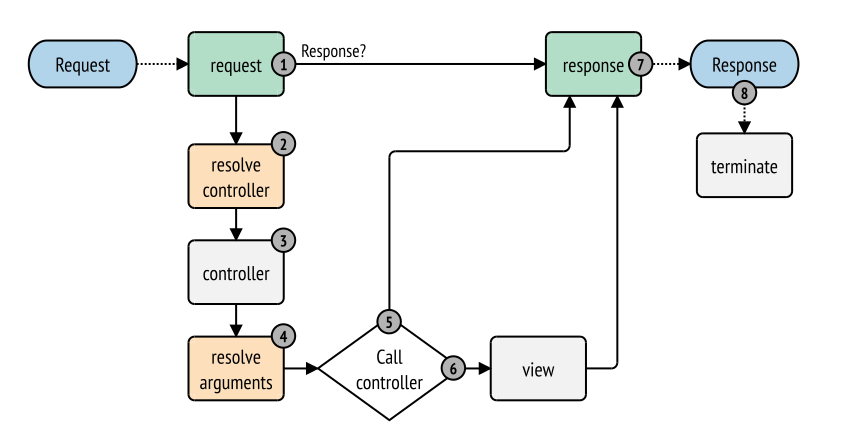
\includegraphics[scale=0.3]{img/http-workflow}
    \caption{Diagrama del proceso de transformación de una petición a una
        respuesta. Fuente:
        \url{https://symfony.com/doc/current/components/http_kernel.html}}
\end{figure}

Cada número representa un paso del proceso, y algunos de estos pasos dispararán
eventos. Al igual que existen eventos, también existen suscriptores a dichos
eventos, que básicamente esperan a que un evento de un tipo determinado se
dispare para realizar una serie de acciones.

\begin{enumerate}
    \item El evento \textit{kernel.request} tiene como objetivo añadir más
        información a la petición \textemdash por ejemplo después de determinar
        en qué idioma debería de darse la respuesta\textemdash, inicializar
        partes del \glslink{webframework}{framework} o crear una respuesta
        inmediatamente y finalizar el proceso: como por ejemplo cuando el
        usuario no tiene la autorización pertinente.
    \item El siguiente paso es averiguar qué controlador ha de llamarse para
        que se ejecute la lógica de negocio acorde a esa respuesta. Esto se
        determina gracias a la información que se extrae de la petición, y a la
        que el programador proporciona al \glslink{webframework}{framework} en
        forma de ciertas directrices como puede ser emparejar una ruta con
        un controlador. Ejemplo: \textit{\"Cuando una petición se realice a la
        ruta /hello/world, se ejecutará la función HelloWorld() del controlador
        HelloWorldController"}.
    \item El evento \textit{kernel.controller} tiene como objetivo preparar la
        ejecución del controlador, ya sea inicializando ciertas partes del
        \glslink{webframework}{framework} o incluso permitiendo que un
        suscriptor cambie el controlador que se va a ejecutar.
    \item En este punto se determinan los argumentos y los valores que han de
        pasarse al controlador. Las formas más comunes de determinarlo suelen
        ser mediante un identificador en la ruta\\ \textemdash
        \textit{/hello/world/argumento1/argumento2}\textemdash, la indicación
        que el programador da para obtener el argumento y finalmente pasando
        directamente la petición al controlador, donde el programador la
        procesará y extraerá los argumentos que le interesen.
    \item Aquí se llama al controlador y se aplica la lógica de negocio
        pertinente según lo que el programador haya programado. En el caso de
        que el controlador devuelva una respuesta, directamente se salta al
        último paso. En caso contrario, se realiza un paso más.
    \item El evento \textit{kernel.view} transforma un resultado de un
        controlador en una respuesta. Aquí es donde suele entrar en juego la
        capa de visualización. Por ejemplo: el controlador devuelve una serie
        de valores que después se insertan en la página correspondiente que
        haya que devolver al usuario, como puede ser el nombre de usuario del
        usuario que realizó la petición.
    \item Finalmente se dispara el evento \textit{kernel.response}, que permite
        a los distintos suscriptores modificar la respuesta antes de que sea
        enviada al usuario.
\end{enumerate}

\subsubsection{symfony/framework-bundle}
La librería encargada de recoger toda la configuración de los diferentes
recursos y elementos que componen el \glslink{webframework}{framework}: las
sesiones, los formularios, validación, enrutamiento\cite{symfony_frambun},
gestión de la capa de visualización, traducciones, cache...

\subsubsection{symfony/security-bundle}
Librería encargada de proporcionar control de acceso a los diferentes recursos
que componen la aplicación. La configuración se realiza mediante parámetros y
patrones de rutas.

\subsubsection{doctrine/orm}
Esta librería provee de \gls{orm} y \gls{dbal} para \gls{php}. Para la
escritura de consultas se utiliza la sintaxis \gls{dql}. He aquí un ejemplo
de una consulta utilizando \gls{dql} y el \textit{Query Builder} de Doctrine:

\begin{minted}[linenos=true]{php}
<?php

$queryBuilder->select('h')
             ->from('house', 'h')
             ->where('h.stories > 2')
             ->orderBy('h.stories', 'ASC');

\end{minted}

\subsubsection{doctrine/annotations}
Esta librería permite realizar anotaciones en las entidades del dominio para
ayudar después a mapear cada atributo y entidad con su tabla y columnas
correspondientes en la base de datos. Un ejemplo de una entidad mapeada podría
ser el siguiente:

\begin{minted}[linenos=true]{php}
<?php

use Doctrine\ORM\Mapping as ORM;

/**
 * @ORM\Entity
 */
class House
{
    /**
     * @ORM\Id()
     * @ORM\GeneratedValue()
     * @ORM\Column(type="integer")
     */
    private $id;

    /**
     * @ORM\Column(type="string", length=255)
     */
    private $name;

    /**
     * @ORM\Column(type="integer")
     */
    private $stories;
}
\end{minted}

\subsubsection{symfony/validator}
Esta librería facilita la validación de los diferentes atributos de las
entidades. La forma de especificación de las restricciones a las cuales están
sujetas, es mediante anotaciones. Así que continuando con el ejemplo anterior:

\begin{minted}[linenos=true]{php}
<?php

use Doctrine\ORM\Mapping as ORM;
use Symfony\Component\Validator\Constraints as Assert;

/**
 * @ORM\Entity
 */
class House
{
    /**
     * @ORM\Id()
     * @ORM\GeneratedValue()
     * @ORM\Column(type="integer")
     */
    private $id;

    /**
     * @ORM\Column(type="string", length=255)
     *
     * @Assert\NotBlank()
     * @Assert\Length(min = 1, max = 255)
     */
    private $name;

    /**
     * @ORM\Column(type="integer")
     *
     * @Assert\GreaterThanOrEqual(0)
     */
    private $stories;
}
\end{minted}

En este simple ejemplo se ha hecho que el atributo \textit{``name''} tenga que
tener una longitud comprendida entre 1 y 255 caracteres, y que el atributo
\textit{``stories''} deba ser mayor o igual que 0. Al quedar las restricciones
plasmadas en la propia entidad, éstas se comprueban para cualquier acceso a
dicha entidad. Por ejemplo, la entidad que se ha usado de ejemplo podría
modificarse mediante un formulario web o una petición a una \gls{api}, pero las
restricciones serán las mismas se modifique de una u otra forma. Huelga decir
que si se requiriese lo contrario, se podría hacer de forma que en el
formulario web se apliquen ciertas restricciones mientras que las llamadas a la
\gls{api} podrían tener restricciones distintas.

\subsubsection{symfony/serializer}
El serializador es un componente que se utiliza para transformar objetos en
formatos específicos, como pueden ser: JSON, XML,
YAML\cite{symfony_serializer}... En el siguiente diagrama se ilustra el
proceso:

\begin{figure}[h]
    \center
    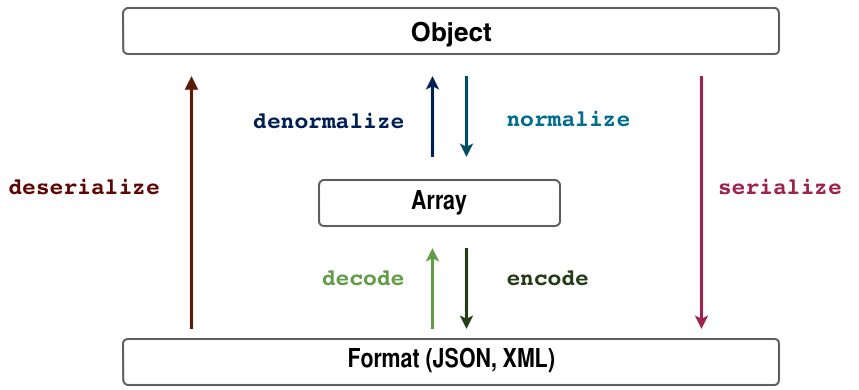
\includegraphics[scale=0.3]{img/serializer_workflow}
    \caption{Diagrama del proceso de serialización de un objeto
      Fuente: \url{https://symfony.com/doc/current/components/serializer.html}}
\end{figure}

Además, mediante el uso de anotaciones, se pueden crear grupos de
serialización, de forma que dependiendo de la petición recibida se pueden
serializar distintos atributos. En el siguiente ejemplo se crean tres grupos,
\textit{private}, \textit{public} y \textit{edit}:

\begin{minted}[linenos=true]{php}
<?php

use Doctrine\ORM\Mapping as ORM;
use Symfony\Component\Serializer\Annotation\Groups;
use Symfony\Component\Validator\Constraints as Assert;

/**
 * @ORM\Entity
 */
class House
{
    /**
     * @ORM\Id()
     * @ORM\GeneratedValue()
     * @ORM\Column(type="integer")
     *
     * @Groups({"private"})
     */
    private $id;

    /**
     * @ORM\Column(type="string", length=255)
     *
     * @Assert\NotBlank()
     * @Assert\Length(min = 1, max = 255)
     *
     * @Groups({"public", "edit"})
     */
    private $name;

    /**
     * @ORM\Column(type="integer")
     *
     * @Assert\GreaterThanOrEqual(0)
     *
     * @Groups({"public"})
     */
    private $stories;
}
\end{minted}

Habiendo etiquetado cada atributo en uno o más grupos de serialización, esto
después puede utilizarse para gestionar de forma dinámica la entidad
dependiendo de las peticiones. Por ejemplo, cuando se hiciera únicamente una
operación de lectura por parte de un cliente sin privilegios, la entidad podría
ser serializada con el grupo \textit{public}, dejando así el atributo
\textit{id} fuera de la respuesta a dar. Lo mismo aplica para los grupos
\textit{edit} que podría utilizarse para limitar las modificaciones a un
atributo en concreto, o el grupo \textit{private} si la casa está siendo
gestionada por un administrador. Los grupos de los nombres en este caso son
esos, pero pueden llamarse como se quiera.

\subsubsection{behat/behat}
Un \glslink{webframework}{framework} \gls{bdd} que permite realizar
\glslink{testsfuncionales}{pruebas funcionales} mediante una sintaxis denominada
\textit{Gherkin}, que facilita la redacción y lectura de las pruebas.
Dichas pruebas se organizan en funcionalidades, escenarios y pasos que después
el \glslink{webframework}{framework} se encarga de ejecutar. Un ejemplo de una
prueba funcional con esta librería podría ser el siguiente:

\begin{minted}[linenos=true]{gherkin}
Feature: House management
  In order to manage houses
  As a house owner
  I need to be able to add a house, modify its parameters or remove it

  Scenario: Modify a house
    Given there exists a house named "My fancy house"
    And I am the owner of it
    When I modify its name to "My beautiful house"
    Then its new name should be "My beautiful house"
\end{minted}

Esta definición de la prueba funcional en \textit{Gherkin} después se mapea a
una clase \gls{php} que interpreta y ejecuta lo que en cada paso debe de
comprobarse:

\begin{minted}[linenos=true]{php}
<?php

class FeatureContext
{
    /**
     * @Given there exists a house named :house
     */
    public function thereExistsHouseNamed($house)
    {
      if(!exists_house($house)) {
        throw new Exception(
          'The house ' . $house . ' doesn't exist'
        );
      }
    }

    /**
     * @Given I am the owner of it
     */
    public function iAmTheOwnerOfTheHouse()
    {
      /** Do stuff */
    }

    /**
     * @When I modify its name to :newName
     */
    public function iModifyItsNameTo($newName)
    {
      /** Do stuff */
    }

    /**
     * @Then its new name should be :expectedName
     */
    public function theNewNameShouldBe($expectedName)
    {
      /** Do stuff */
    }
}
\end{minted}
Este ejemplo se ha simplificado para facilitar la asimilación del concepto
detrás de \textit{Behat}. Una vez hechos los mapeos correctamente
\textit{Behat} se encargará de ejecutar las funciones, y en caso de que no
produzcan ningún error los pasos correspondientes se considerarán como
correctos.

\subsubsection{justinrainbow/json-schema}
Librería utilizada para validar objetos JSON con \textit{JSON Schema}. Por
ejemplo, imaginemos que al realizar una petición al servidor para
obtener información sobre una entidad \textit{House}, dicho servidor devuelve
lo siguiente:
\begin{minted}[linenos=true]{json}
{
  "id": 1,
  "name": "My beautiful house",
  "stories": 2
}
\end{minted}
A la hora de realizar las pruebas de la aplicación, la información que devuelva
el servidor puede ser variada, a pesar de que el entorno de pruebas cargue una
serie de casas predefinidas. En vez de validar que el JSON que devuelve el
servidor es exactamente igual a las diferentes casas que existen en la base de
datos \textemdash porque recordemos que en vez de devolver un único objeto
\textit{House}, el servidor podría devolver un \textit{array} de ellos
\textemdash, se puede comprobar que el objeto JSON devuelto es válido acorde a
un esquema. Por ejemplo:

\begin{minted}[linenos=true]{json}
{
  "type": "object",
  "properties": {
    "id": {"type": "integer"},
    "name": {
      "type": "string",
      "pattern": "^[a-zA-Z0-9]+$"
    },
    "stories": {
      "type": "integer",
      "minimum": 0
    }
  },
  "required": ["id", "name"]
}
\end{minted}
Este esquema, que ha obviado algunos elementos para simplificar el ejemplo,
podría utilizarse para validar las diferentes respuestas que puede dar el
servidor con respecto a diferentes casas. Esto puede resultar muy interesante
para reducir el tamaño de las pruebas y concentrar en un único esquema las
condiciones del objeto JSON que el servidor debería de enviar.

\subsubsection{lexik/jwt-authentication-bundle}
Esta librería provee de una implementación de los \gls{jwt}: Esta tecnología
es un estándar abierto\footnote{\url{https://tools.ietf.org/html/rfc7519}} que
define una forma compacta y autocontenida \textemdash debido a que el token
tiene toda la información del usuario y no es necesario volver a consultar a la
base de datos \textemdash de intercambiar
información entre dos entidades mediante un objeto JSON. Además, la información
puede ser verificada debido a que se firma digitalmente bien utilizando un
secreto, bien utilizando claves públicas y privadas. \cite{jwt_explanation}

Como se ha comentado anteriormente, \gls{jwt} tiene una naturaleza compacta y
autocontenida. Esto es realmente útil, por ejemplo, en arquitecturas \gls{rest}
donde no hay estados: debido a que cada llamada a una \gls{api} \gls{rest} debe
de contener toda la información necesaria para que el servidor pueda procesarla
correctamente, los tokens \gls{jwt} son extremadamente útiles para transmitir,
por ejemplo, la información respecto al usuario que está realizando dicha
llamada. De esta forma el servidor puede extraer todos los datos del token para
comprobarlos y autorizar o no el procesamiento de la petición realizada. He
aquí un diagrama explicando el proceso de inicio de sesión:

\begin{figure}[h]
    \center
    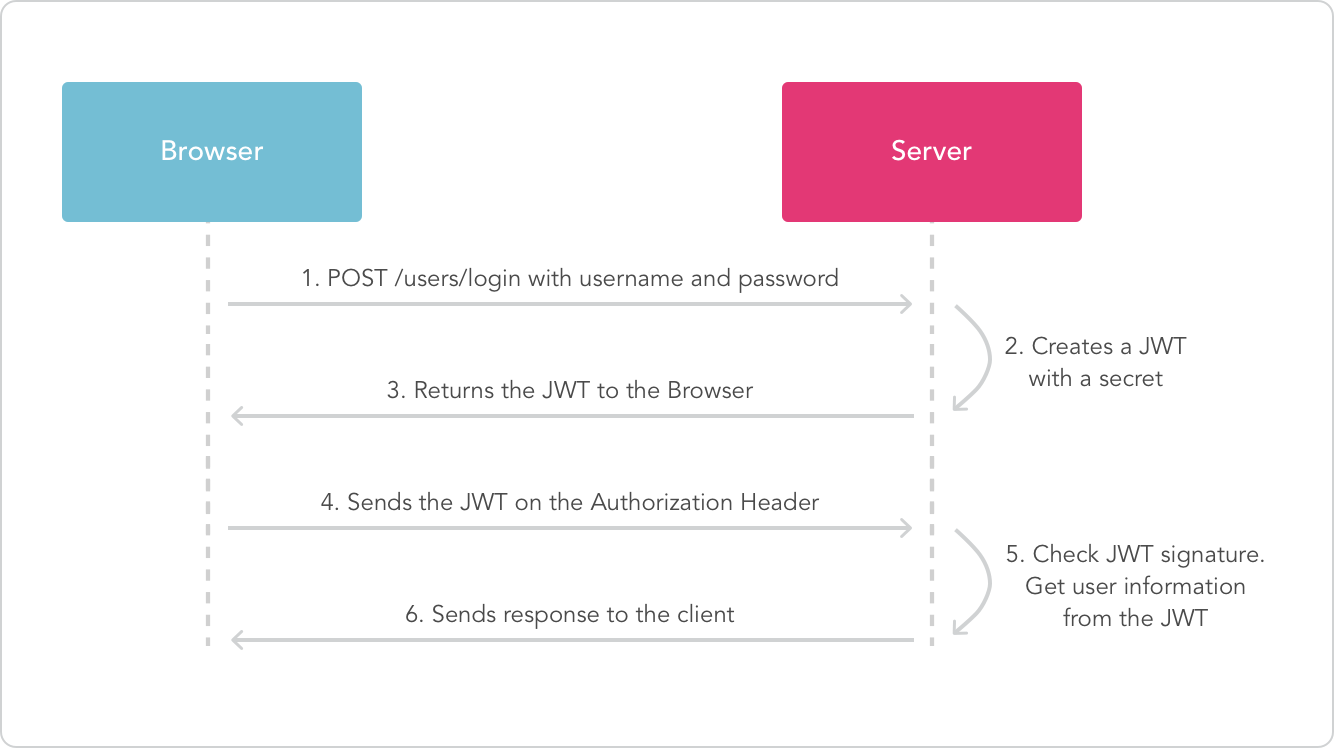
\includegraphics[scale=0.3]{img/jwt-diagram}
    \caption{Diagrama del proceso de inicio de sesión mediante un token
      \textit{JWT}. Fuente:
        \url{https://jwt.io/introduction/}}
\end{figure}

Tal y como se ve en el diagrama, el token \gls{jwt} se envía adjuntado en cada
petición, en una de las cabeceras de la misma: la cabecera
\textit{Authorization}.

\subsubsection{api-platform/api-pack}
Este es un metapaquete el cual agrupa otras librerías que dan la funcionalidad
necesaria para incorporar API Platform en una instalación estándar de Symfony.
Entre otras librerías, incluye \textit{api-platform/core}, que es la librería
que al fin y al cabo provee de las funcionalidades indicadas en la sección de
\glslink{webframework}{frameworks} \ref{tech:apiplat}.


\section{Clepsydra, la aplicación}
\subsection{Arquitectura de la aplicación}
\subsubsection{Servidor}
El servidor donde la aplicación iba a ser probada para su funcionamiento era
una máquina virtual GNU\\Linux que iba sobre una capa de
virtualización \gls{kvm}. Básicamente la empresa ya tenía \gls{kvm} montado y
simplemente tuve que configurar dicho servidor, adhiriéndome a los parámetros
que el informático de sistemas me facilitó.

\subsubsection{Sistema operativo}
El sistema operativo que escogí para montar el servidor fue Debian. El motivo
es que he utilizado mucho la susodicha distribución, y por lo tanto pensé que
sería mucho más fácil configurar una máquina utilizando una tecnología que ya
conocía. Debido a que en la empresa estaban de acuerdo con ello, fue finalmente
la que utilicé.

La distribución se clasifica principalmente en tres ramas: \textit{stable},
\textit{testing} y \textit{unstable}, y debido a que quería ahorrarme
quebraderos de cabeza en el futuro escogí la rama estable de la distribución.

No obstante, debido a su naturaleza estable, algunos de los paquetes que
requería \textemdash principalmente \gls{php} \textemdash no estaban en la
versión que ciertas librerías de la aplicación requerían, por lo que realicé
un pequeño ajuste con lo que se denomina \textit{apt-pinning}.

\textit{apt-pinning} se realiza cuando se precisa obtener versiones de
paquetes, o paquetes enteros, que no están en la rama de la distribución
actual. De esta forma se pueden obtener paquetes determinados en una versión
más moderna, permitiendo así tener las virtudes de un sistema en un estado
estable junto con las modernidades específicas de ciertos paquetes.

Esto se realizó después de comprobar que la primera opción recomendada,
los \gls{backports}{backports} para los paquetes necesarios, no estaban
disponibles por aquel momento.

\subsubsection{Base de datos}
Para la base de datos de la aplicación se utilizó \textit{MariaDB}, que es un
\glslink{fork}{fork} del proyecto de base de datos relacional \textit{MySQL}.
No se concibió utilizar una tecnología de base de datos diferente debido a
que no se esperaba que la aplicación fuera a gestionar un volumen y un tráfico
de datos que no fuera fácilmente manejable por una base de datos relacional. No
merecía la pena sacrificar ninguno de los principios \gls{acid}, ni tampoco un
\gls{rdbms} que proveyera del cumplimiento de los mismos, por una hipotética
necesidad de rendimiento y escalabilidad que fuera a requerir de un paradigma
de base de datos diferente.

El diagrama del \glslink{modentrel}{modelo entidad-relación} que usa la
aplicación se puede encontrar en la figura \ref{fig:erdiag}. La idea general es
que la aplicación podrá gestionar clientes, que a su vez agruparán proyectos
en grupos de proyectos. Cada proyecto puede categorizarse, y además puede tener
bolsas de horas \textemdash una especie de presupuesto en la que el cliente
consume horas de la susodicha bolsa de horas \textemdash y presupuestos. Los
proyectos predefinidos tienen como fin el ser una plantilla de la que copiar
los proyectos que son comunes a distintos grupos de proyectos. Los usuarios
pueden asignarse a proyectos, y además son los que crean las diferentes tareas
en cada proyecto. Las tareas favoritas tienen el mismo objetivo que los
proyectos predefinidos: facilitar la creación de tareas que se repiten
obteniéndolas de una lista previamente creada.

Este esquema se creó a raíz de las diferentes reuniones que se mantuvieron con
los interesados, en las cuales se debatió el modelo de gestión que tenían
decidido utilizar, y que dieron como fruto el esquema de la figura
\ref{fig:erdiag} que solventa y refleja las necesidades que se me expusieron.

Además, se puede observar que muchas de las entidades únicamente tienen un
par de campos: el identificador y el nombre. Esto es consecuencia de haber
consultado con los gestores sobre la adición de nuevos campos en las entidades,
que resultaran útiles para definir dichas entidades aún mejor. Pero en el
software que utilizaban no les daban un uso significativo, y tampoco preveían
que les fueran a dar más uso en esta aplicación. Por lo tanto decidí prescindir
de ellos e invertir el tiempo en otras tareas, pero manteniendo la estructura
del dominio de forma que si nuevos campos tuvieran que ser añadidos en el
futuro, algo que sí preveía probable, se pudiera hacer sin tener que
reestructurar el modelo.

\begin{figure}[p]
    \center
    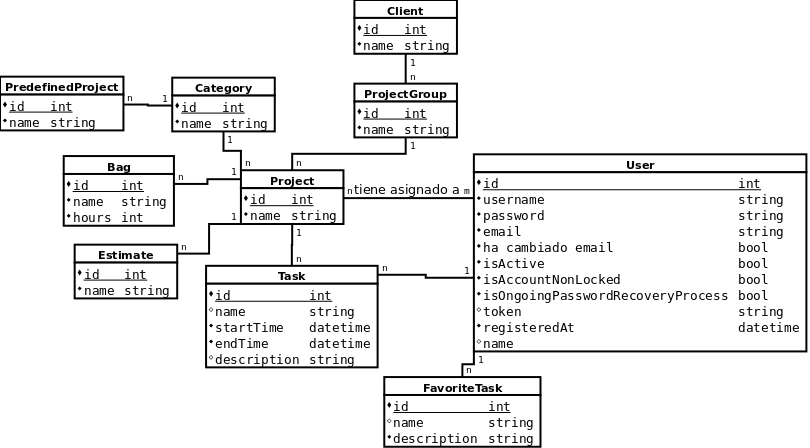
\includegraphics[angle=90,scale=0.6]{img/erDiagram}
    \caption{Diagrama del modelo entidad-relación de la base de
datos\label{fig:erdiag}}
\end{figure}

\subsubsection{Roles}
\label{sec:roles}
Por deseo de los interesados, los usuarios de la aplicación se iban a dividir
en tres grupos principales: gestor con privilegios, gestor, y usuario normal.
En la figura \ref{fig:useCases} se pueden apreciar los diferentes casos de uso
asignados a cada rol. También se puede observar que los roles se heredan, y por
lo tanto el gestor con privilegios heredará los casos de uso del gestor regular
y el usuario regular.

\begin{figure}[p]
    \center
    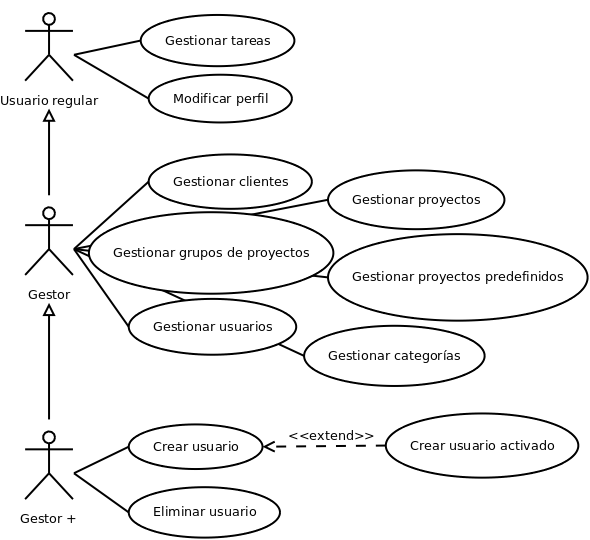
\includegraphics[scale=0.6]{img/useCase}
    \caption{Diagrama de casos de uso de la aplicación}
    \label{fig:useCases}
\end{figure}

\paragraph{Usuario regular}
El usuario con menos privilegios de la aplicación. La idea de este rol es que
los usuarios tengan la sensación de que sólo ellos están utilizando la
aplicación, y por lo tanto, se restringe el acceso a toda la información que no
tenga que ver directamente con él, y por lo tanto puede \textemdash por
gestionar se entiende crear, modificar y eliminar\textemdash:

\begin{itemize}
    \item Consultar su perfil de usuario.
    \item Modificar sus datos de usuario.
    \item Modificar su email y verificarlo.
    \item Modificar su contraseña.
    \item Recuperar la contraseña.
    \item Consultar los proyectos en los que toma parte \textemdash indicándole
        el nombre, grupo del proyecto y la categoría del mismo \textemdash.
    \item Gestionar tareas en los proyectos a los que está asignado.
    \item Gestionar sus tareas favoritas.
\end{itemize}

\paragraph{Gestor}
El gestor es el usuario con privilegios al que se le permite acceder y
modificar casi cualquier apartado de la aplicación. En la siguiente lista
se listan las funcionalidades a las que tiene acceso:

\begin{itemize}
    \item Gestionar clientes.
    \item Gestionar grupos de proyectos y asignarlos a clientes.
    \item Gestionar proyectos y asignarlos a grupos de proyectos, y también
        categorizarlos.
    \item Abrir y cerrar proyectos: de esta forma ningún usuario puede imputar
        más tareas al proyecto.
    \item Gestionar proyectos predefinidos. Además, los proyectos creados a
        partir de un proyecto predefinido verán sus campos modificados si un
        gestor modifica el proyecto predefinido al que está relacionado.
    \item Gestionar categorías.
    \item Gestionar bolsas de horas y asignarlas a proyectos.
    \item Gestionar presupuestos y asignarlos a proyectos.
    \item Gestionar las tareas de cualquier usuario de la aplicación.
    \item Gestionar las tareas favoritas de cualquier usuario de la aplicación.
    \item Modificar el perfil de cualquier usuario de la aplicación.
    \item Activar y desactivar un usuario, lo que permite restringirle por
        completo el acceso a la aplicación.
    \item Asignar y revocar el acceso de los usuarios a los proyectos.
\end{itemize}

\paragraph{Gestor con privilegios}
El gestor con privilegios es el usuario que puede utilizar la aplicación sin
ningún tipo de restricción. Los interesados del proyecto insistieron en que
únicamente un rol específico debería de poder añadir y eliminar usuarios de la
aplicación, ya que opinaban que eso facilitaría la gestión de la misma. Así que
las funcionalidades que se le ofrecen a los usuarios con este rol son:

\begin{itemize}
    \item Crear un usuario en la aplicación.
    \item Eliminar un usuario de la aplicación.
\end{itemize}


